\chapter{Lecture 4}
\subsection{N-Arity}
$\bar{Z_{n}} = [1...n]$

\subsubsection{}An n-ary address space A is a subset of $\Bar{Z^{*}_{n}}$ that is prefix closed if $q: A$ and $p$ is a prefix of q, then $p: A$.\\

Example:
\begin{figure}[htbp]
    \center
    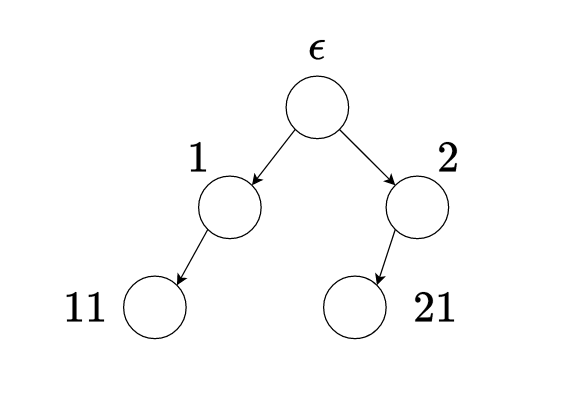
\includegraphics[scale=0.8]{images/popl-4-1.png}
    \caption{}
\end{figure}

$A = {\epsilon, 1, 2, 11, 21}$
\subsubsection{}
Let A be an n-ary address space and let $p:A$ .
\begin{gather}
    A@p = \{q: \bar{Z_{n}^{*}}\  \vert\  pq: A\}  \xrightarrow{} \text{Address space of A relative to p}
\end{gather}

e.g.
\indent $A@2 = \{\epsilon, 1\}$

\subsubsection{}
Context at p (excluding p)
\begin{gather}
    C_{ex}(A, p) = A\backslash pA@p\\
    \xrightarrow{} \text{concatenating p with each address (in subtree) relative to p}
\end{gather}

Context at p (including p)
\begin{gather}
    C_{in}(A, p) = C_{ex}(A,p) \cup \{p\}
\end{gather}
\begin{figure}[htbp]
    \center
    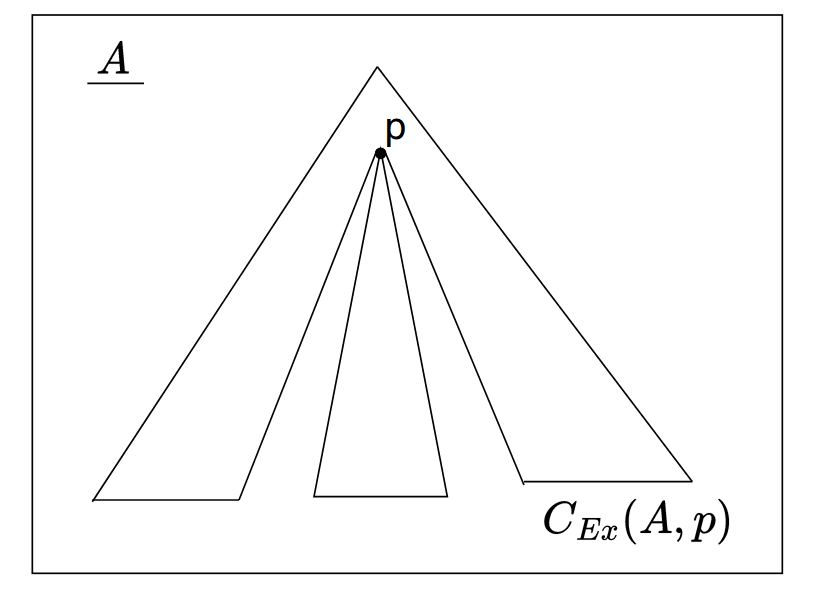
\includegraphics[scale=0.5]{images/popl-4-2.png}
    \caption{}
\end{figure}

\subsection{Terms, Subtrees, Tree Contex}
\subsubsection{}
Let A be an address space. A term is a map $t:A\xrightarrow{}v$ where $V$ is a set of values.

Example:
\begin{gather}
    V = \mathcal{N}, A = \{\epsilon, 1, 2\}\\
    t: \{\epsilon\xrightarrow{}5, 1\xrightarrow{}7, 2\xrightarrow{}7\}
\end{gather}

\begin{figure}[htbp]
    \center
    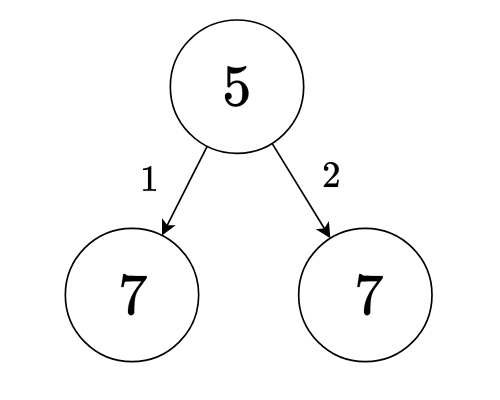
\includegraphics[scale=0.6]{images/popl-4-3.png}
    \caption{}
\end{figure}

\subsubsection{}
Let $t:A\xrightarrow{v}$ be a tree and let $p:A$
\begin{gather}
    C_{ex}(t,p) = df = t \vert_{C_{ex}(A,p}
\end{gather}

\subsubsection{}
Let $\Sigma_{s}$ be a set of symbols.\\
Let $\alpha: \Sigma_{s} \xrightarrow{ \mathcal{N}}$ denote the arity map of $\Sigma_{s}$.\\

Example,\\
\begin{gather}
    \Sigma_{s} = \{f,a,b\}
    \alpha_{s}: \{f\xrightarrow{}2, a\xrightarrow{}0, b\xrightarrow{}0\}\\
    \implies f(a,b) \checkmark \ \ \ \ a \checkmark \ \ \ \ b \checkmark \ \ \ \ f(a) \times
\end{gather}

\subsubsection{}
A term is $(A,\Sigma_{s}, \alpha, t: A\xrightarrow{} \Sigma_{s})$\\
s.t.
\begin{enumerate}
    \item A is a prefix-closed language over $\mathcal{N}_{+}$
    \item $\forall p: A$, if $t_{p}=S$ and $\alpha(S)=n$\\
    then $p1,..., p\alpha(S): A$ \ \ \ \ \  \ \ \ 
    $\forall i: 1 \leq i \leq \alpha(S), pi: A, \forall i: \mathcal{N}_{+}\backslash[1,...,\alpha(S)]pi\notin A$
\end{enumerate}
\newpage
